\documentclass[man, floatsintext, 10pt]{apa6}
% floatsintext so that figures show up where we want them to (https://www.tug.org/pracjourn/2012-1/beitzel/beitzel.pdf)
\usepackage{lipsum}
\usepackage{amsmath}
\usepackage{harmony}  % Music stuff % https://martin-thoma.com/how-to-write-music-with-latex/
\usepackage{dirtytalk} % Quote


\PassOptionsToPackage{hyphens}{url}\usepackage{hyperref}
\usepackage[american]{babel}
\usepackage{ulem}
\usepackage{graphicx}
\usepackage{csquotes}
\usepackage[style=apa,sortcites=true,sorting=nyt,backend=biber]{biblatex}
\DeclareLanguageMapping{american}{american-apa}

\title{fakesAreBAye}

\shorttitle{fakesAreBAye}

\author{Sean Pili and Pedro Uria \\ Bayesian Methods for Data Science}

\affiliation{GWU}

\begin{document}
\maketitle

\section{Introduction}

In this project, we develop models via Bayesian and Machine Learning methods in order to tell whether a restaurant review is real or fake, as well as to analyze various predictors that play or do not play a role in the matter. This problem is of great interest to both the consumer and the food service industry because a great majority of people read restaurant reviews online in order to make a well-informed decision on their meal destination. These reviews greatly affect consumers' prior beliefs about a particular business, and, unfortunately, it has been known for a while that some of these businesses pay individuals to write fake reviews, either positive towards their own products and services, or negative towards their competitors. This immoral activity hurts consumers who may trust these fake reviews, even when they may be wary of them, because at first glance and even under careful inspection, fake reviews can very well look like real reviews. In order to take this into account, we use a combination of text and behavioral features based on the reviewers previous activities.  While we focus on restaurants, this work could be extended to other kinds of reviews, such as hotels, services, and products in general.

A good amount of work has previously been done in this matter. Mukherjee et. al used a combination of behavioral and n-gram features to predict whether Yelp reviews for restaurants and hotels were real or fake. They achieved an accuracy of 82.8 \%, recall of 87.9 \% and precision of 82.1 \% using behavioral features alone. When adding n-grams, they increased their accuracy to 84.1 \%, their precision to 83.4 \%, but their recall fell to 87.1 \%. Barbado et. al  extended their work, using their own behavioral features and linguistic features, as well as well as metadata about the reviewer accounts from an e-commerce website to predict whether the e-commerce reviews were fake and achieved an F1 score of 82 \%. Maajar et. al used behavioral data and metadata about reviewers only to achieve a recall of 91 \% when using them to classify android and IOS apps as real or fake. 

Obviously, the only way to train a classifier to detect fake reviews is to know whether each review the model is trained on is real or fake. Of the review platforms we  searched in our literature review, only Yelp makes fake reviews public. That is to say, Yelp publishes whether its internal algorithm detected whether a given review is real or fake. Scraping the reviews was a tedious task, so we asked Mukherjee et. al to send us the Yelp data they used for their analysis and they were kind enough to do so. 

\section{Data}

\paragraph{Raw data} The dataset we used was collected by Mukherjee et. al in order to analyze Yelp's review filter. It consists of  $61,541$ reviews of restaurants located in Chicago that were scraped from Yelp's website, and includes the review itself, together with the date, a unique review id, reviewer id, product id, star rating and label. 53,400  of the reviews were real and  8,141 were fake, leaving us with an imbalanced dataset with the minority class making up 13 percent of the data. The star rating ranges from 1 to 5, and only has integer values. Each review was automatically labeled as either real or fake by Yelp's filter algorithm. While this ground truth may not be completely accurate, Yelp is bold enough to make the fake reviews public, meaning that they have a great amount of trust on their model, which has also been under study and deemed to be fairly precise by Mukherjee et. al. It is worth noting that Yelp has access to additional private user data, which is most likely being used to improve their system. The goal of our project is thus to provide other companies with a baseline of how to implement a fake review filter algorithm, as well as analyze the public features that are most relevant to this problem. 

Upon further inspection of the data, we noticed that many of the users had only one review, which made calculating the maximum cosine similarity among user reviews for one user impossible, and make all of the features that incorporate averages less meaningful. Therefore, we dropped all users from the dataset that only had one review. After doing this, the dataset contained 37,936 reviews, 35,850 of which were real, and 2,086 were fake, meaning we had a very imbalanced dataset with the minority class, fake reviews, making up only 5.8 percent of our data. 

\vspace{2mm}

\paragraph{Behavioral Features} Mukherjee et. al extracted 5 behavioral features, all of which we used in our analysis. The first feature we used was MNR, or the maximum number of reviews a user has posted in a day. The authors state that 75 percent of spammers wrote 6+ reviews a day when looking across both their restaurant and hotel datasets (i.e. the first quartile of the MNR variable was 5), but in our restaurant dataset, the first quartile for MNR is 1. Furthermore, the 90th percentile of MNR is 2, meaning that 90 percent of the reviewers writing fake reviews wrote at most 2 or fewer reviews per day. It could be possible that the restaurant dataset is much smaller than the hotels dataset and the spammers in the hotel dataset wrote many more fake reviews per day.  Oddly, the 75th percentile of MNR is actually higher for non-spammers (2), than spammers (1), meaning that a higher percentage of genuine reviewers are writing more reviews per day than spammers. Although the difference may be negligible, it is strange that the trend the paper discusses is reversed in the restaurant dataset. The second behavioral feature, PR, is the percentage of user ratings that are 4 stars or higher. Mukherjee et. al reported that 85 percent of spammers rated more than 80 percent of their reviews positive, and that roughly 50 percent of regular reviewers rated reviews as positive across both restaurants and hotels combined.  However, in our restaurant dataset, the median of the PR variable is .5 for both spammers and non-spammers. The third behavioral feature is average review length, which is much longer for real reviewers than fake reviewers in the literature when considering both restaurants and hotels.  The fourth behavioral feature is reviewer deviation, which is calculated as follows: the average star rating is calculated for each productID (aka restaurant ID) in the dataset, the absolute deviation from that average rating is calculated for every reviewer that reviewed that product. That process is repeated for every product in the dataset. After that, an average is taken across those deviations for each reviewer in the dataset. So, if a spammer gave three restaurants that have an average rating of three stars ratings of 5, 5 and 4 stars, their reviewer deviation statistic would be 4.67. This variable's summary statistics differ with those described in our literature review. Although in both cases, the reviewer deviation for spammers is higher than that non-spammers, it is not higher to the extreme  mentioned in the literature review. I.e. 80 percent of the real reviewers had a reviewer deviation of greater than .45 as opposed to .69 for spammers in our dataset, but in the literature review, 80 percent of the fake reviewers had a reviewer deviation of greater than 2.5 and and 80 percent of real reviewers had a reviewer deviation greater than .6. The final behavioral feature is maximum cosine similarity (mcs) between reviews of a given reviewer. They did not specify if any pre-processing such as tokenization, lemmatization or stemming was applied to the text before cosine similarity was calculated, so we do not expect the summary statistics of that variable to match Mukherjee et. al's exactly. For reference, we tokenized the text with NLTK and applied the porter stemmer to the tokens. However, we again find it odd that the average cosine similarity of spammers is lower than the cosine similarity  of the real reviewers, because Mukherjee et. al reported the opposite results.
 \vspace{2mm}
 
\paragraph{Text Features} For computing the text features, we decided to use a state-of-the-art Neural Network called BERT, which will be briefly explained in the next section. We do not delve into this part very deeply, as we are aware that not even a human can distinguish well-crafted fake reviews from genuine reviews based on the text alone.


\section{Modeling}

In this section we discuss the models we used to tackle this problem. This is a binary classification task, in which we want to be able to correctly label an online restaurant review as either real or fake. We have discussed the previous work and incorporated the behavioral features used in our literature review into our own models. However, we have taken a new approach for the text features.

\vspace{2mm}

\paragraph{BERT} In our case, we used BERT as a language feature extractor. BERT is a Neural Network that has achieved state-of-the-art results in many NLP tasks, including classification. Although describing this language model is not of interest here, and thus will be treated as a black box, it is noteworthy that the authors have a lot of experience using BERT-like models. The input to these models can be thought of as raw text for the purpose of this work, and in order to extract the features for each review, we add a linear layer on top of BERT, that maps its 768-dimensional output to a 3-dimensional dense vector, and another linear layer with a sigmoid output function that maps this vector to the probability of a review being real or fake. Therefore, once BERT is trained by minimizing a Binary Cross-Entropy performance index on our training data to classify the reviews, we go forward on our test data and use the intermediate 3-dimensional vector output as our text features. 

Regarding the specifics of training BERT, we decided to cut the reviews at 100 tokens long, as BERT's time complexity is quadratic to the sequence length; and if the text actually reveals whether a review is real or fake, we speculated such pattern would also be present in the first one hundred words. We only used the first 4 layers of this model (each layer has the same architecture as the final layer and the same number of output dimensions), a batch size of 32 reviews, and the Adam weight-decay optimizer with a learning rate of $e^{-5}$ and an epsilon of $e^{-8}$. In order to force the features to be more meaningful towards fake reviews, we weighted our loss during training using the proportion of real vs fake reviews. All the training was done in PyTorch and we used the huggingface transformers implementation of BERT, starting from its base uncased pre-trained version.

\vspace{2mm}

\paragraph{Bayesian Logistic Regression} Once all the features were ready, we proceeded to train logistic regression models under the Bayesian probabilistic approach using R and JAGS. In order to do so, we had to give prior distributions to each of the parameters in our logistic regression equation before we ran the MCMC sampling process that allows us to infer their posteriors. Such priors will be discussed in the next section. In regards to the specific bayesian model, we use the following hierarchical approach 

\[\beta_i \sim \text{ Normal distribution} \] \[ \uparrow \] 
\begin{equation} 
\label{Bern} 
 \mu = \frac{1}{1 + e^{-\big(\beta_0 + \sum_i \beta_i x_i \big)}} 
 \end{equation}
\vspace{0.01mm}  \[ \uparrow \] \[ y \sim\ \text{bernoulli} (\mu) \]

in which the target variable follows a Bernoulli distribution, with its probability following the logistic equation. Each of the logistic coefficients also follow the prior distributions mentioned above. By the iterative Markov-Chain Monte-Carlo algorithm, we sample from the posterior distributions of each of our coefficients until the chains converge. For a more detailed explanation of the theory behind this learning process, you can read \textit{Doing Bayesian Analysis} by John K. Kruschk. We also experiment with more advanced methods such as Robust Logistic Regression, which helps to deal with outliers by incorporating into the model a small chance ($\alpha/2$) of a data point being randomly generated, and variable selection, in order to deal, for the most part, with the BERT features. Variable selection is achieved by multiplying each logistic coefficient by a binary variable $\delta_i$. Thus, if this multiplier is 0, the feature $i$ will not be used in the model. Of course, these new parameters also need priors, which come from Bernoulli distributions with different probabilities, chosen to be above 0.5 because we start from the assumption that every feature is important. The most general model we used is therefore described as follows:

 \[\beta_i \sim \text{ Normal distribution}, \hspace{2mm} \delta_i \sim \text{ Bernoulli distribution}, \hspace{2mm}\  \alpha \sim \text{ Beta distribution (1, 9)} \] \[ \uparrow \] \[ \mu = \frac{1}{2} \alpha + (1 - \alpha) \frac{1}{1 + e^{-\big(\delta_0 \beta_0 + \sum_i \delta_i \beta_i x_i \big)}} \] \vspace{0.01mm}  \[ \uparrow \] \[ y \sim\ \text{bernoulli} (\mu) \]
 
In the next section we elaborate on different priors and their posteriors, the use of the advanced approaches, and our inference results.

\section{Experiments and Results}

\paragraph{Overview} Although most of the experimental work focused on running MCMC, we also experimented when training BERT, until we got a decent model by using the approach mentioned at the beginning of the previous section. Such model reported a recall of 88 \%, meaning that 88 out of 100 fake reviews were identified, while the overall accuracy was 43 \%. That is, BERT also labeled a bit more than half of the real reviews as fake. We forced BERT to act this way to have more relevant features towards identifying fake reviews. The experiments prior to these results will not be discussed as they are not relevant for this work. We decided to keep the number of BERT features very small compared to the original size (3 vs 768), in order to avoid overwhelming the likely more important behavioral features, and also to reduce the MCMC running time. While we standardized the behavioral features, we did not do so for BERT's, because they were already within a [-2, 2] range (see figure \ref{BERTf}), and doing so would mess with our approach for choosing the priors (explained in the next paragraph). We conducted several experiments in order to arrive at well-behaved chains. In this section we explain the most relevant of those experiments, as well as present and analyze our results. 

\vspace{2mm}

\paragraph{Priors} Even though the cdfs of our features did not agree with Mukherjee et. al's, we still decided to use the relationships present in their research to choose the initial values of our priors. For reviewer deviation, PR, MNR and cosine similarity we chose normal distributions with mean of 1 and standard deviation of $2^{-2}$, which means that we expected higher values of these features to make it more likely for a review to be fake. On the contrary, a larger average review length would be expected to decrease the probability of a review being fake, so the mean was chosen to be -1, while the standard deviation was kept the same.

Regarding the BERT features, we decided to go with normal distributions, using the BERT weights as means. That is, on our final classification layer, we basically have the following equation: $\text{prob}_{\text{fake}} = \text{sigmoid} (w_0 p_0 + w_1 p_1 + w_2 p_2 + b)$, where $p_i$ is our feature $i$ and $w_i$ is its weight. Given the fact that the sum inside the sigmoid is exactly a part of the sum inside our bayesian model, using the $w_i$ as the mean for the $p_i$ priors is likely the best we can do, even more so when realizing that we do not know what the BERT features really represent. We also use the bias as the mean for our intercept's prior normal distribution, for the very same reason. The bias and weights were $0.021997$ and ($-0.5015929$, $-0.3729589$, $0.3562961$). 

\vspace{2mm}

\paragraph{Posteriors} For all the experiments, we run 3 MCMC chains with different but constant random seeds and initializations, using JAGS for 15,000 steps. The specifics hyper-parameters to reproduce our results can be found in our GitHub \href{https://github.com/seanpili/-fakesAreBAye/blob/master/RecurrentUsers/experiments.txt}{repository}. We started with the basic bayesian logistic regression approach but soon switched to the combination of the robust and variable selection improvements. All the experiments we will discuss are based on this advanced approach. Unless explicitly mentioned, we used 0.5 delta for the intercept and 0.9 for the rest of the features, and a guess multiplier of 0.2. Our first thought was to include all the features we had computed, which resulted in very bad convergence for most of them. When we looked at the correlation, we realized the cosine similarity was very correlated with these features, so we decided to exclude it from our next experiments. Afterwards, we re-run MCMC and all the features had good convergence except for the first two BERT features, as shown in figure \ref{BERTfMCMC}. This was actually to be expected given the huge correlation among these features, as evidenced by figure \ref{BERTf}. Therefore, we decided to also drop the first two BERT features. In doing so, we also found that PR and MNR were not significant, as we can see in the posteriors shown in figure \ref{PR_MNR_Posteriors}. Figure \ref{PR_MNR_Deltas} shows the deltas for such features, which further confirms the little predictive power of PR and MNR. This agrees with our EDA.

\begin{figure}
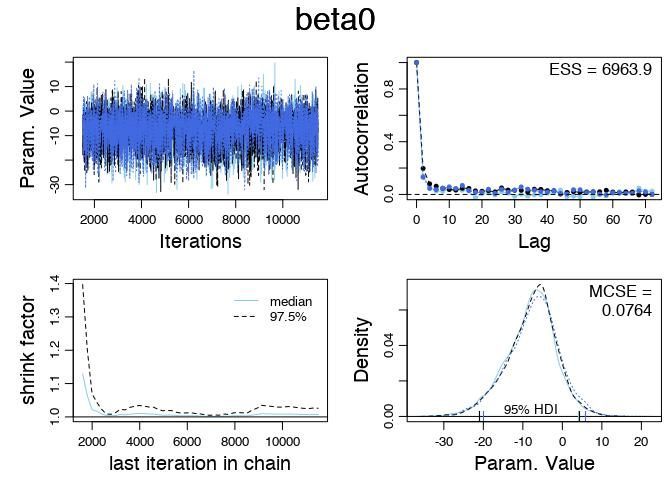
\includegraphics[width=8cm]{Intercept_exp1.jpg}
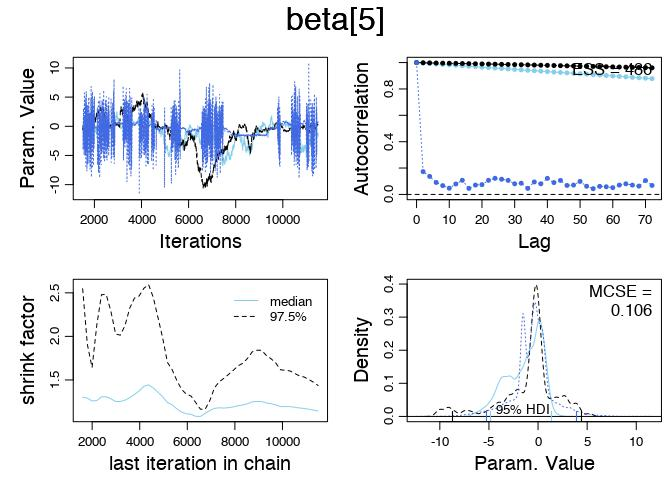
\includegraphics[width=8cm]{BERTf1_exp1.jpg} \\
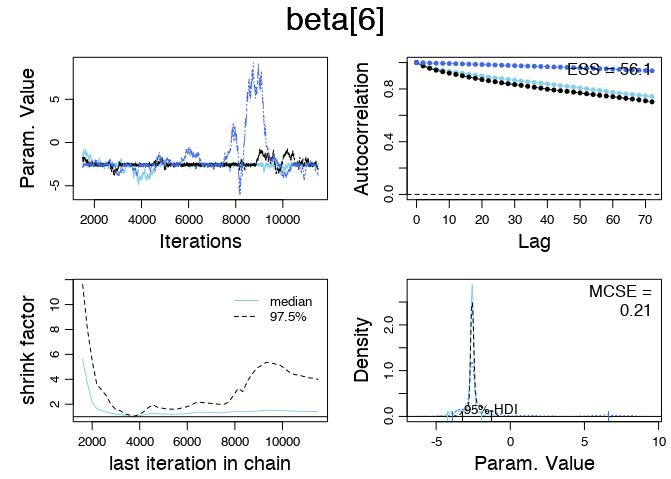
\includegraphics[width=8cm]{BERTf2_exp1.jpg}
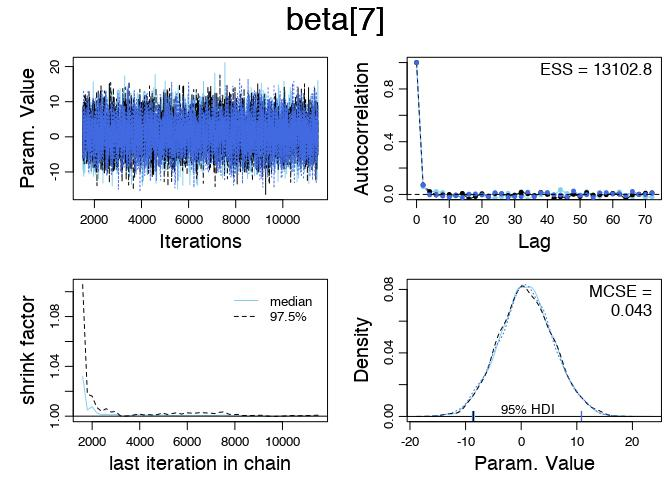
\includegraphics[width=8cm]{BERTf3_exp1.jpg}
\caption{Intercept (beta0) and BERT's features MCMC convergence}
  \label{BERTfMCMC}
\end{figure}

\begin{figure}
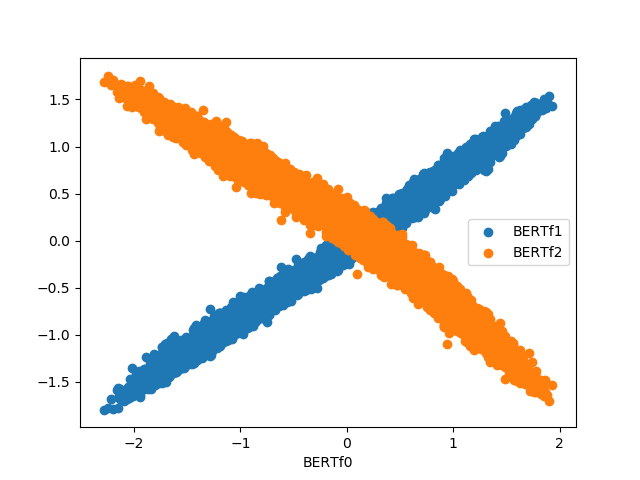
\includegraphics[width=8cm]{BERTFeaturesScatterPlot.png}
\caption{BERT's features scatter plot}
  \label{BERTf}
\end{figure}

\begin{figure}
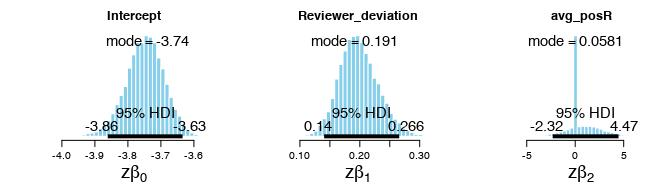
\includegraphics[width=8cm]{posteriors_bdata_02.jpg}
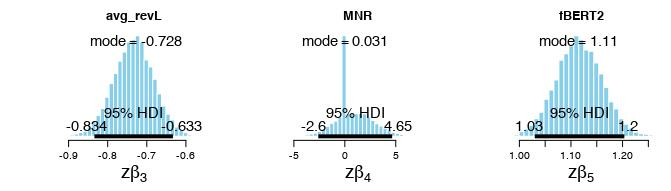
\includegraphics[width=8cm]{pposteriors_bdata_02.jpg}
\caption{PR and MNR Posteriors from Experiment \#3}
  \label{PR_MNR_Posteriors}
\end{figure}

\begin{figure}
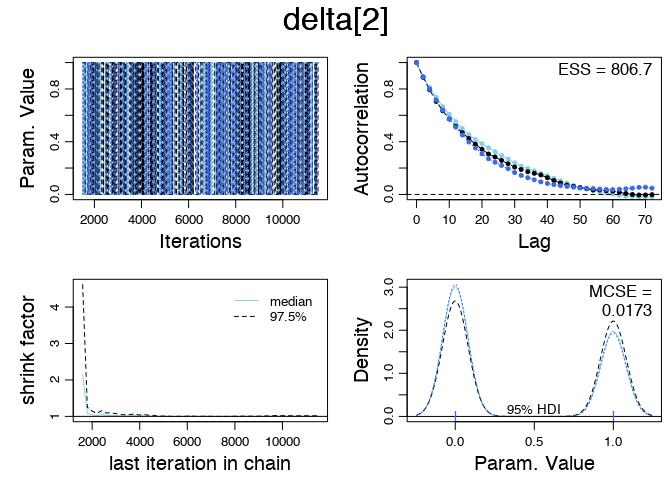
\includegraphics[width=8cm]{delta_PR_bdata_02.jpg}
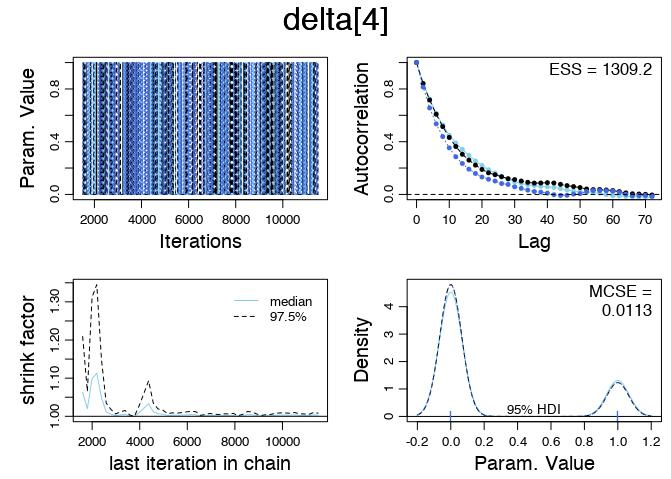
\includegraphics[width=8cm]{delta_MNR_bdata_02.jpg}
\caption{PR and MNR Deltas from Experiment \#3}
  \label{PR_MNR_Deltas}
\end{figure}

\begin{figure}
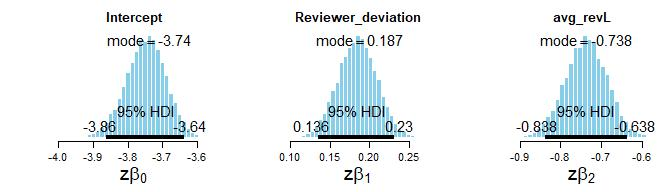
\includegraphics[width=8cm]{posteriors_bdata_03.jpg}
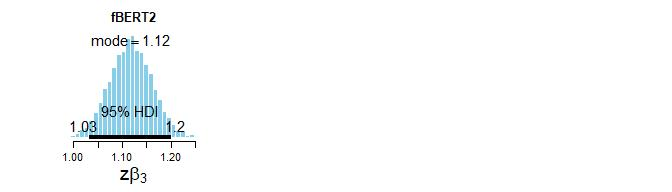
\includegraphics[width=8cm]{pposteriors_bdata_03.jpg}
\caption{Posteriors from Experiment \#4}
  \label{Exp4}
\end{figure}

\begin{figure}
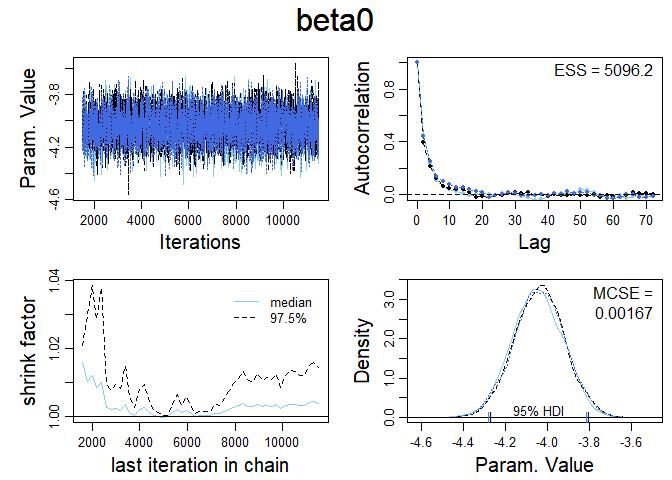
\includegraphics[width=8cm]{Intercept_exp4.jpg}
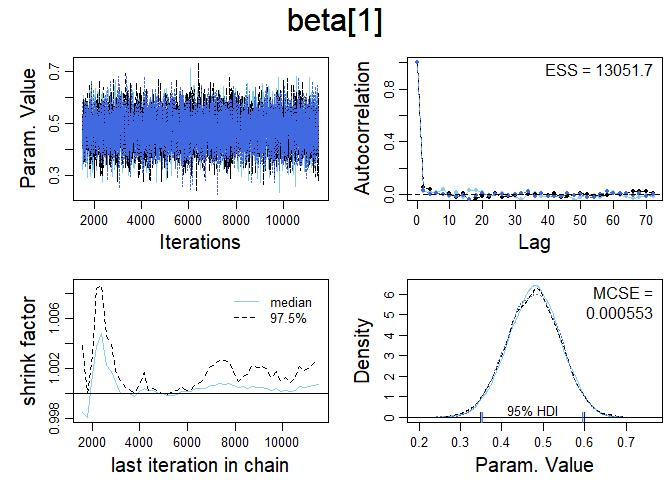
\includegraphics[width=8cm]{ReviewerDevExp4.jpg} \\
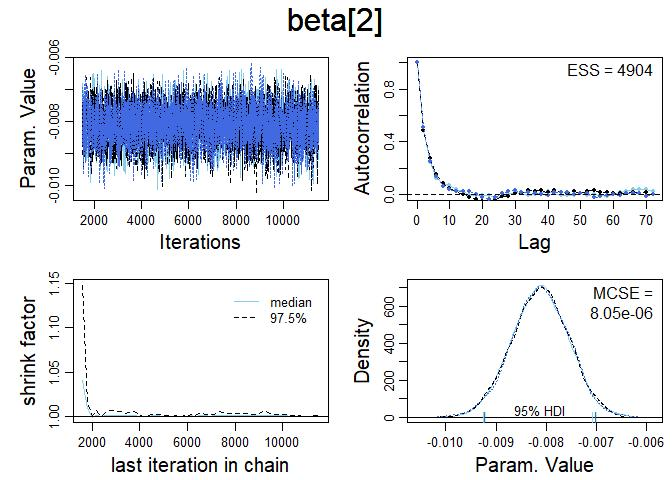
\includegraphics[width=8cm]{AvgRevLenExp4.jpg}
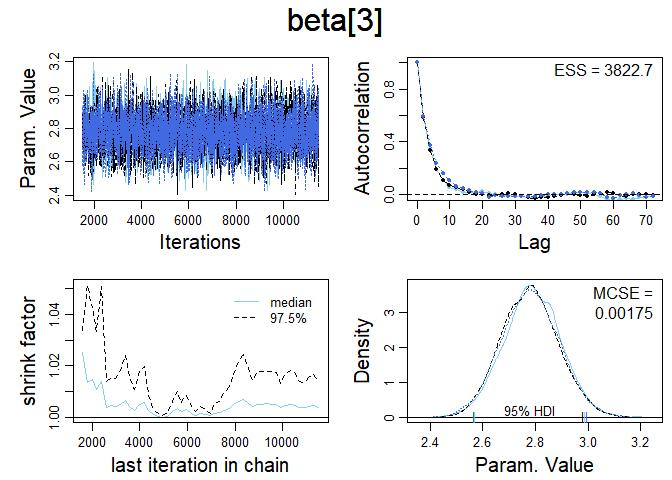
\includegraphics[width=8cm]{BERTExp4.jpg}
\caption{MCMCs from Experiment \#4}
  \label{Exp4MCMC}
\end{figure}

\begin{figure}
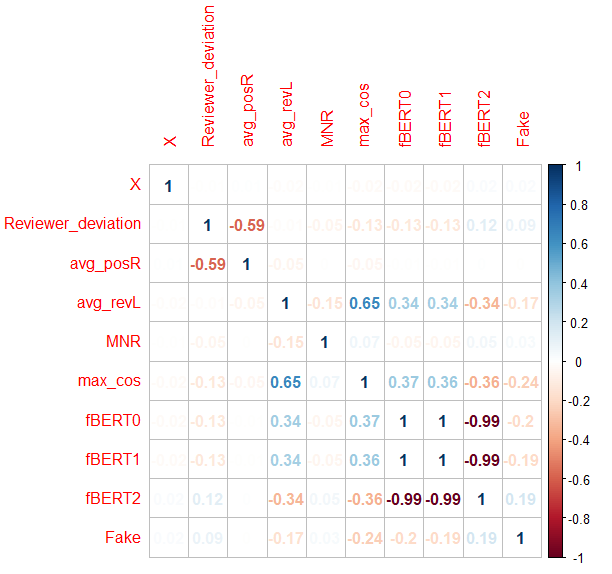
\includegraphics[width=8cm]{corrplot.png}
\caption{Correlation Matrix Between Features}
  \label{corr}
\end{figure}

corrplot

Finally, we decided to also drop these two features, and re-run the MCMC. This time, we get modes outside of the HDI for all features (figure \ref{Exp4}), with that HDI itself being pretty narrow, and the convergence is also very good (figure \ref{Exp4MCMC}). In particular, the standardized Reviewer Deviation mode is 0.187, which means that the probability of a review being fake increases slightly when this feature increases. On the other hand, the mode for average review length per user is -0.738, meaning that the probability of a review being fake decreases when the user who wrote it writes longer reviews, which was also the expected behavior. BERT's mode is 1.12, and while we cannot really interpret it, it seems BERT did a good job extracting some kind of info from the text alone that allows to help distinguish between real and fake reviews. Last but not least, the intercept's mode is -3.74, which has the highest absolute value and tells us that the model gives anyone the benefit of the doubt, which is desired.

However, we note that our remaining features are still correlated (figure \ref{corr}), which makes this kind of mode analysis not ideal. We tried to include an interaction term 

.... TODO .... Our best and final experiment .... I guess we should be able to remove some individual feature terms .... TODO ....

\vspace{2mm}

\paragraph{Prediction Methods} We experimented with a variety of methods in order to use our Bayesian Logistic Regression to classify the reviews in our test set. The first method was to use the mode of the MCMC-generated beta samples as our coefficients (but first rounding the samples to 2 decimal places because there could be infinitely many continuous beta values), and substitute in equation \ref{Bern}. For the second method, we removed the Bernoulli likelihood from that equation and simply applied a threshold, starting at 0.5 (reviews with probabilities greater or equal than 0.5 are labeled as fake). The latter approach typically generated higher accuracy than the former approach with thresholds between .4-.6 because values generated from a Bernoulli distribution will be 1 or 0 as long as the probability of success is not exactly 0 or 1. I.e., even though the outputs of the logistic equation of our Betas and the data may output values close to 1 or 0, such as .9 or .1, which are synonymous to outputting very confident predictions that reviews are real or fake, using those values as the probability of success in a Bernoulli trial to generate our final prediction will occasionally yield counter-intuitive final predictions. Although the thresholding approach yielded higher accuracy than using Bernoulli trials, the recall from both methods was similar using a threshold of .5. However, we could increase recall by lowering the threshold. TODO: Make sure this is the case

Another method we used to generate predictions was as follows: first, we would apply equation \ref{Bern} to each set of N betas generated from the MCMC and apply thresholding (with values between .1 and .9) to generate N predictions for each row in the test set, and then use majority voting to yield the final prediction for each row in the test set. This method was typically less accurate than using only the mode of the betas to make predictions and applying thresholding to the output of the logistic equation, but it generated much higher recall using an accuracy of .5. TODO: Make sure this is the case. The final method was taking the mean of the output logistic equation for each sample and only apply the threshold on this mean. TODO: Results on this.

\paragraph{Final results} ..... TODO .....

\section{Conclusions} 

TODO https://arxiv.org/pdf/1903.12452.pdf

https://link.springer.com/article/10.1007/s10664-019-09706-9
\end{document}

